\documentclass[11pt,a4paper]{article}
\usepackage[margin=2.4cm]{geometry}
\usepackage{amsmath,amssymb}
\usepackage{booktabs}
\usepackage{graphicx}
\usepackage{float}

\graphicspath{{../outputs/}}

\setlength{\parindent}{0pt}
\setlength{\parskip}{6pt}

\title{\textbf{Lab: Root of a Nonlinear Equation}\\[4pt]
\large Newton--Raphson Method and Secant Method}
\author{}
\date{}

\begin{document}
\maketitle
\vspace{-3em}

\section*{Objective}
To find the real root of the equation $x\log_{10}x=1.2$ using both the
Newton--Raphson method and the secant method, correct to five decimal places.

\section*{Formulae Used}

\textbf{Newton--Raphson method.} Starting from an initial approximation $x_{0}$,
\begin{equation*}
x_{n+1} \;=\; x_{n}-\frac{f(x_{n})}{f'(x_{n})}, \qquad n=0,1,2,\ldots
\end{equation*}

\textbf{Secant method.} Starting from two initial approximations $x_{0}$ and $x_{1}$,
\begin{equation*}
x_{n+1} \;=\; x_{n}-f(x_{n})\,\frac{x_{n}-x_{n-1}}{f(x_{n})-f(x_{n-1})},
\qquad n=1,2,3,\ldots
\end{equation*}

The iteration is stopped when successive approximations agree to five decimal
places, i.e.\ when $\lvert x_{n+1}-x_{n}\rvert<\tfrac{1}{2}\times10^{-5}$.

\section*{Newton--Raphson Solution}
Let $f(x)=x\log_{10}x-1.2$. Since
$\dfrac{d}{dx}\bigl(x\log_{10}x\bigr)=\log_{10}x+\log_{10}e$, we have
\[
f'(x)=\log_{10}x+0.434294 .
\]
Take $x_{0}=404$. The iteration is
\[
x_{n+1}=x_{n}-\frac{x_{n}\log_{10}x_{n}-1.2}{\log_{10}x_{n}+0.434294}.
\]

\begin{center}
\begin{tabular}{cccccc}
\toprule
$n$ & $x_{n}$ & $\log_{10}x_{n}$ & $f(x_{n})$ & $f'(x_{n})$ & $x_{n+1}$ \\
\midrule
0 & 404.000000 & 2.606381 & 1051.778072 & 3.040676 & 58.097272 \\
1 & 58.097272  & 1.764156 & 101.292635  & 2.198450 & 12.022708 \\
2 & 12.022708  & 1.080002 & 11.784552   & 1.514297 & 4.240513 \\
3 & 4.240513   & 0.627418 & 1.460576    & 1.061713 & 2.864834 \\
4 & 2.864834   & 0.457100 & 0.109514    & 0.891394 & 2.741977 \\
5 & 2.741977   & 0.438064 & 0.001161    & 0.872358 & 2.740646 \\
6 & 2.740646   & 0.437853 & 0.000000    & 0.872147 & 2.740646 \\
\bottomrule
\end{tabular}
\end{center}

At the sixth iteration $x_{6}=2.740646$ and $x_{7}=2.740646$ agree to five decimal
places, so the process is stopped. Hence
\[
\boxed{x \approx 2.74065}
\]

\section*{Secant Solution}
Take $x_{0}=404$ and $x_{1}=405$ (the same far starting region used for
Newton--Raphson) and apply the secant iteration to the same
$f(x)=x\log_{10}x-1.2$.

\begin{center}
\begin{tabular}{cccccc}
\toprule
$n$ & $x_{n-1}$ & $x_{n}$ & $f(x_{n-1})$ & $f(x_{n})$ & $x_{n+1}$ \\
\midrule
1 & 404.000000 & 405.000000 & 1051.778072 & 1054.819284 & 58.158355 \\
2 & 405.000000 & 58.158355  & 1054.819284 & 101.426938  & 21.259500 \\
3 & 58.158355  & 21.259500  & 101.426938  & 27.023114   & 7.858012 \\
4 & 21.259500  & 7.858012   & 27.023114   & 5.835378    & 4.167068 \\
5 & 7.858012   & 4.167068   & 5.835378    & 1.382876    & 3.020719 \\
6 & 4.167068   & 3.020719   & 1.382876    & 0.250279    & 2.767402 \\
7 & 3.020719   & 2.767402   & 0.250279    & 0.023392    & 2.741285 \\
8 & 2.767402   & 2.741285   & 0.023392    & 0.000558    & 2.740648 \\
9 & 2.741285   & 2.740648   & 0.000558    & 0.000001    & 2.740646 \\
\bottomrule
\end{tabular}
\end{center}

At the ninth iteration $x_{9}=2.740648$ and $x_{10}=2.740646$ agree to five decimal
places, so the process is stopped. Hence
\[
\boxed{x \approx 2.74065}
\]

\section*{Comparison}
\begin{figure}[H]
\centering
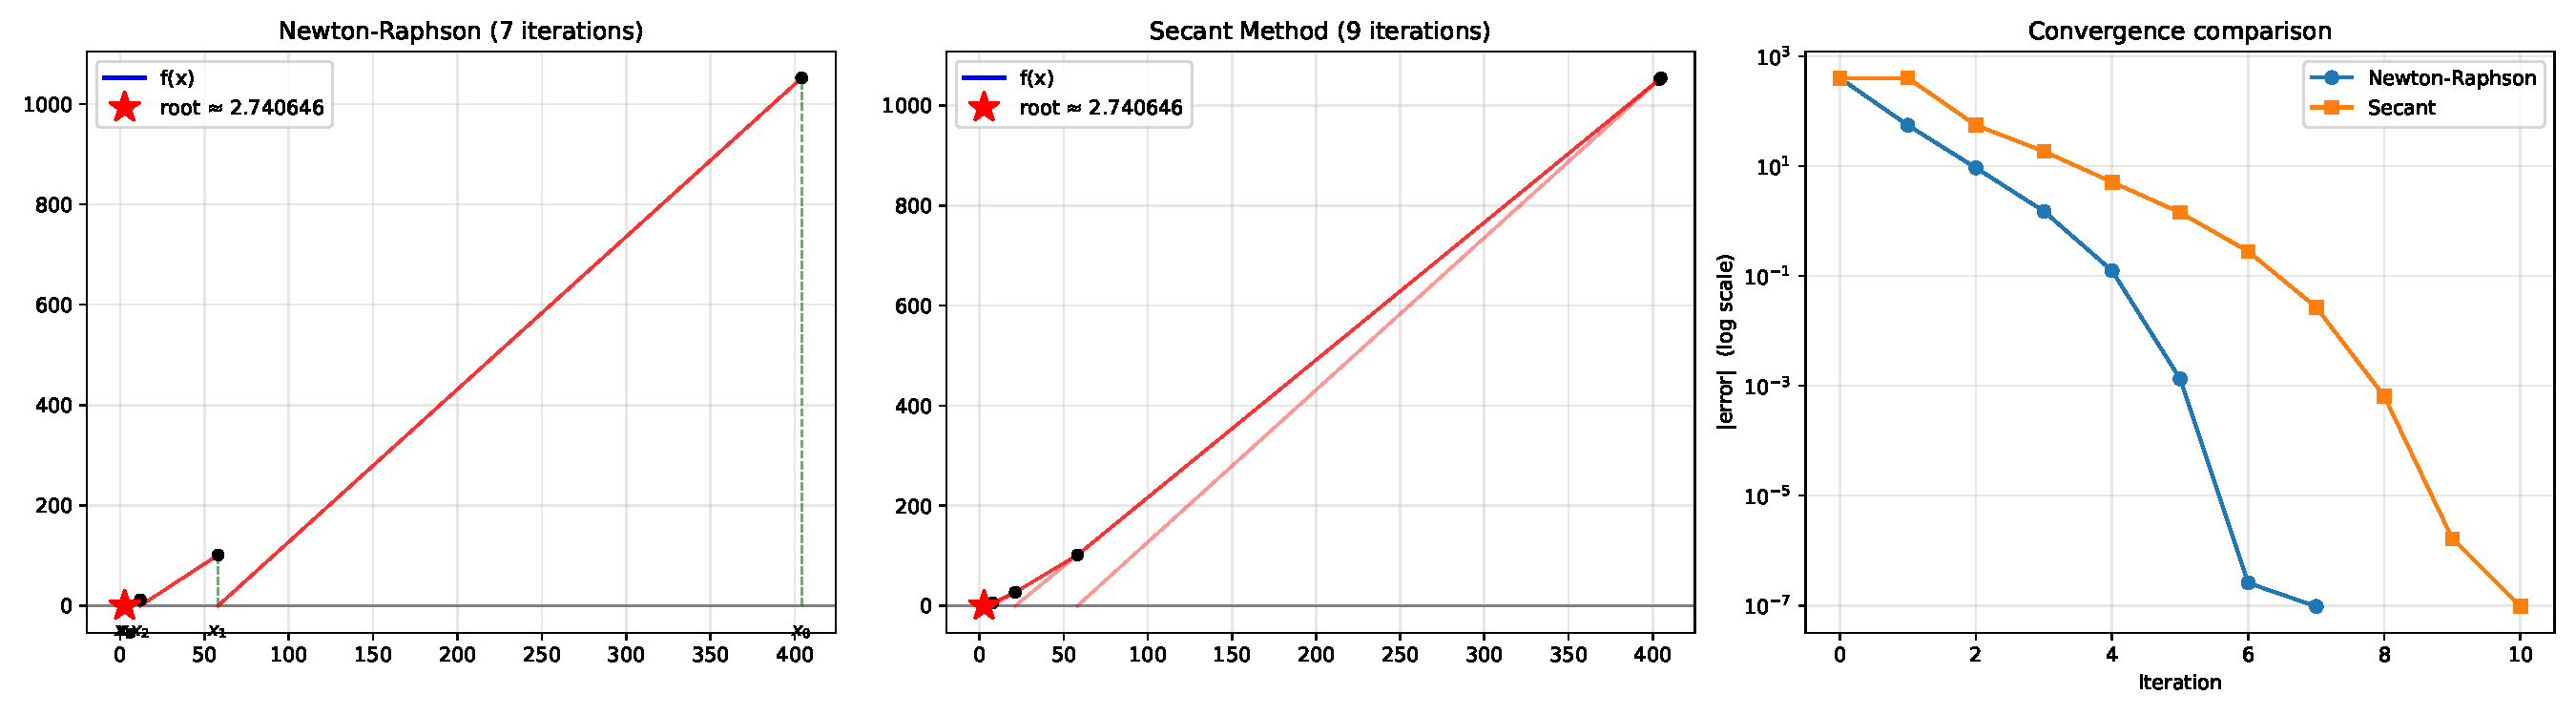
\includegraphics[width=0.78\textwidth]{problem3_methods.pdf}
\caption{The curve $f(x)=x\log_{10}x-1.2$ near the root, showing the
Newton--Raphson iterates (circles) and the secant iterates (squares) both
converging to $x\approx2.740646$. Both methods are started from the same far
region ($x\approx404$); their very large early steps fall off-window and are
omitted for clarity.}
\end{figure}

\section*{Conclusion}
Both methods converge to the real root $x\approx2.74065$ (correct to five decimal
places). Here both were started from the same far region --- Newton--Raphson from
$x_{0}=404$ and the secant method from $x_{0}=404,\;x_{1}=405$ --- so their
iteration counts may be compared directly. From this identical starting region
Newton--Raphson reaches five-decimal accuracy in \textbf{7} iterations, while the
secant method needs \textbf{9}.

The difference reflects their orders of convergence once near the root.
Newton--Raphson converges \emph{quadratically}: the error falls
$1.2\times10^{-1}\to1.3\times10^{-3}\to2.6\times10^{-7}$, roughly squaring at each
step. The secant method converges \emph{superlinearly} with order $\approx1.618$:
the error falls
$2.8\times10^{-1}\to2.7\times10^{-2}\to6.4\times10^{-4}\to1.6\times10^{-6}$. Thus
Newton--Raphson is faster in iteration count, but each of its steps additionally
requires an evaluation of the derivative $f'(x)$; the secant method needs no
derivative and pays for this only with a slightly lower order of convergence and,
here, two extra iterations.

\end{document}